\documentclass{article}
\usepackage[utf8]{inputenc}
\usepackage{geometry}
\usepackage{graphicx}
\usepackage{hyperref}

\geometry{
left=25mm,
right=25mm,
top=20mm,
bottom=25mm
}

\title{\textbf{Report N°4 MSc Thesis: Active Constraints}}
\author{\textbf{Alberto Rota} - \textit{Supervisor: Prof. Elena De Momi}}
\date{}

\begin{document}
\maketitle
\paragraph{Title:} \textit{To Be Defined}
\section*{General guidelines}
    Development of surgical training tasks implementing Active Constraints of
    different nature and with different levels of intervention, in order to
    evaluate their efficacy and role in Robot-Assisted Minimally Invasive Surgery.
    \begin{itemize}
        \item \textit{Phase 1: }Software Development in a virtual environment (Unity)
        
        Construct a number of surgical tasks that implement Active Constraints on Unity. "Active
        Constraints/Virtual Fixtures: A survey"
        \href{https://ieeexplore.ieee.org/document/6634270}{(link here)} is being used as a guide of the workflow and as a point of reference.
        \item \textit{Phase 2: }Implementing on the dVRK, followed by
        experimental tests with data gathering, analysis and validation
        
        The tasks will be implemented and connected on the dVRK in the lab, and the virtual PSM in the tasks will be controlled by the manipulator. Then, the scope of the thesis is to gather a number of subjects (volunteers) that will perform the tasks with and without the virtual fixtures in order to evaluate the efficacy of the Active Constraints. 
    \end{itemize}

\section*{Work Planned from the previous report}
\begin{itemize}
    \item Literature research on surgical tasks: what to aim at and what to
    focus on when building one
    \item From the rudimentary task alredy implemented, create more complex
    ones that will allow to employ the different types of virtual fixtures.
    \newline NOTE: Anywhere possible, the virtual objects employed will be 3D models
    of organs, and the end-effector will be replaced by the PSM tooltip
\end{itemize}

\section*{Progress}
\begin{itemize}
    \item Information about the task (reference trajectory, position/velocity of the PSM over time, force over time, position of the obstacles, \textit{etc.}) are now logged automatically and consistently on \textit{.csv} files, in order to compare them easily
    \item Built two fully functional surgical tasks which implement 3D models of real organs, a PSM and trajectories of real surgical operations (one task is a Nephrectomy, the other one is a Liver Resection). In the e-mail where this report is attached I'm also uploading two videos of me performing the tasks:
    \begin{itemize}
        \item \texttt{video\_for\_ke\_trajectoy.mp4}: A Trajectory Guidance Virtual Fixture is employed, aiding the user in guiding the PSM along the green trajectory in green. The first trial is performed without the Virtual Fixture, and the second one is performed with it (you can see a blue force pulling toward the trajectory). Below, a figure with the post-processing of the results shows the reference trajectory, the PSM trajectory and the force vector: this is a 3D plot.
        \item \texttt{video\_for\_ke\_surface.mp4}: A Surface Guidance Virtual Fixture is employed, aiding the user in slicing a lobe of the liver while remaining on the plane shown as the green disc. Here, I recorded only the trial with the Virtual Fixture activated. A blue force is clearly pulling the PSM towards the surface when the user is getting too far. Below, a figure with the post-processing of the results shows the reference surface, the PSM trajectory and the force vector: this is a 3D plot
    \end{itemize}
    At the moment, I am piloting the PSM with AWSD keys on my keyboard, for testing purposes. Also, the tasks can be become more complex and articulated, maybe combining multiple sub-tasks: I've coded everything so that it would be easy to combine multiple Virtual Fixtures.

    I will add "target points" in the tasks: the task will be completed once the user reaches all the target points.

    All of the material I've been working on is on my GitHub at: \newline \textbf{\href{https://github.com/alberto-rota/MSc-Thesis-Active-Constraints-in-RAMIS}{https://github.com/alberto-rota/MSc-Thesis-Active-Constraints-in-RAMIS}} (but some files are not under version control, e-mail me if you need any more clarification)

\end{itemize}

\section*{Next Steps}
\begin{itemize}
    \item Build more tasks employing the other types of Virtual Fixtures that have already been implemented (at least one task for Virtual Fixture)
    \item Start planning the structure for written report of the thesis (I will write a previsionary "Table of contents")
\end{itemize}

\newpage
\section*{Screenshots}
The quality of the images here is not the best, I'm aware of that.
    \begin{figure}[h!]
        \begin{small}
            \begin{center}
                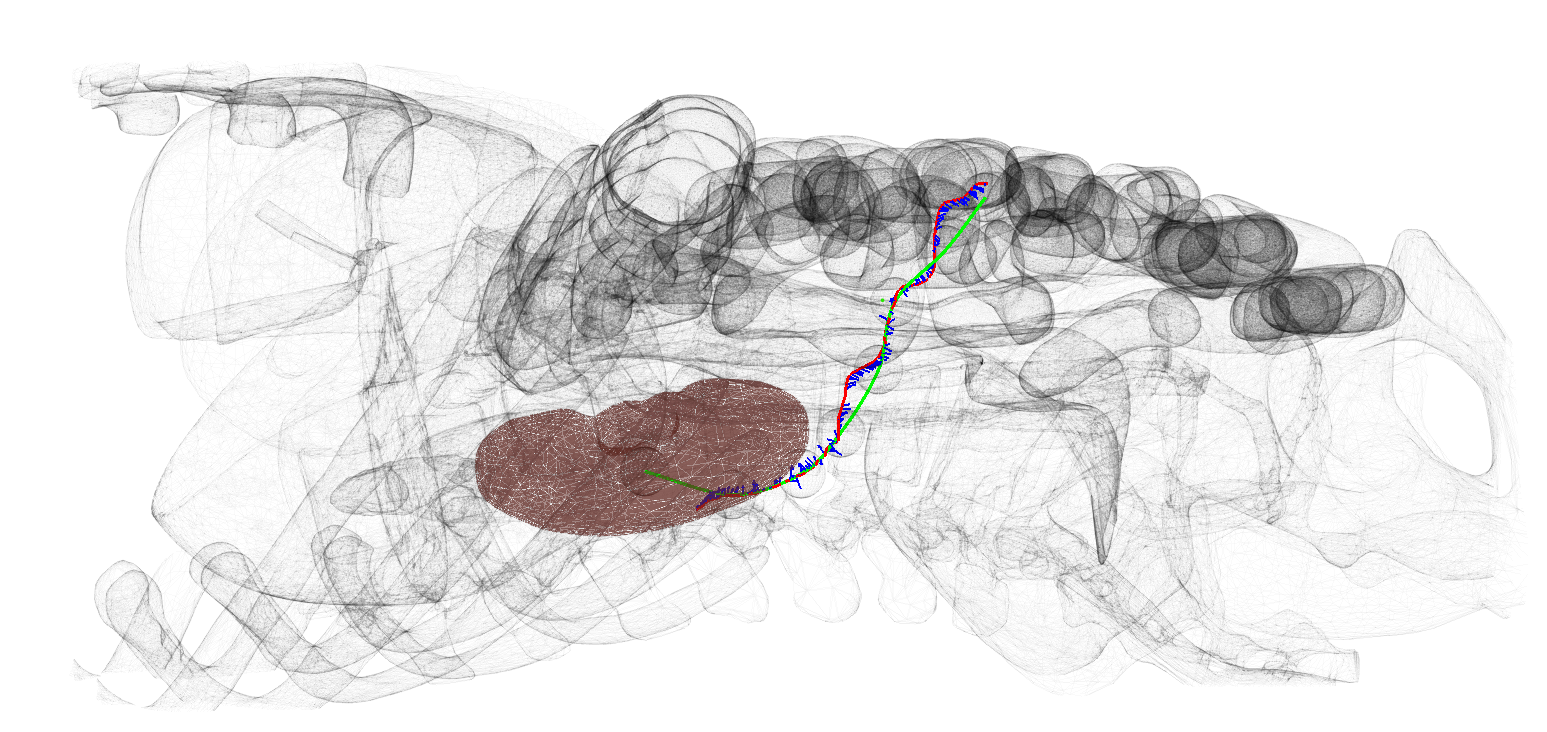
\includegraphics[width=0.9\textwidth]{trajectory.png}
            \end{center}
            \caption{Post-processing of the Nephrectomy task}
        \end{small}
    \end{figure}
    \begin{figure}[h!]
        \begin{small}
            \begin{center}
                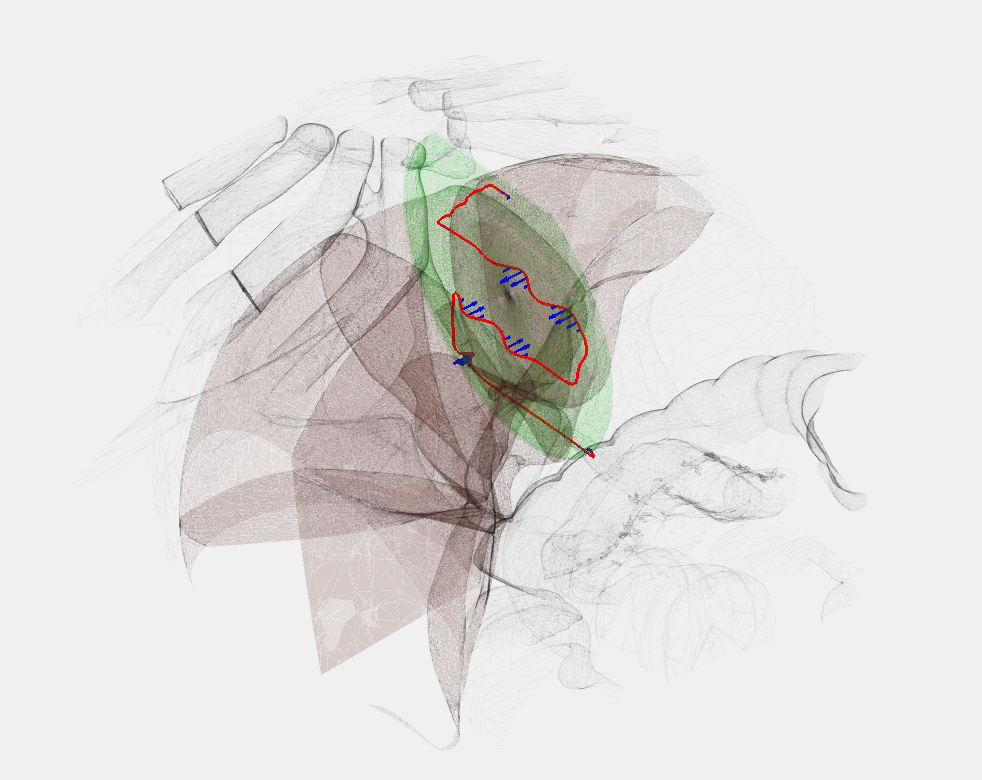
\includegraphics[width=0.65\textwidth]{surface.png}
            \end{center}
            \caption{Post-processing of the Liver Resection task}
        \end{small}
    \end{figure}

    
\end{document}